\chapter{Análisis y diseño de la solución}
\label{cha:AnalysisAndDesign}

En este capítulo se hablará del análisis y del diseño adoptado para resolver el problema de generar chatbots. Para ello, como se ha mencionado previamente, se ha definido un artefacto llamado SheetChat. En el Apartado \ref{sec:Requisitos} se hablará de los requisitos que ha de tener el artefacto que permita generar bots. En el Apartado \ref{sec:FeatureModel} se realizará el análisis de las funcionalidades que ha de tener SheetChat. Finalmente, en el Apartado \ref{sec:DataModel} se mostrará cual es el modelo de datos a definir para la generación de agentes conversacionales basados en hojas de cálculo.

\section{Requisitos}
\label{sec:Requisitos}



\section{Modelo de características}
\label{sec:FeatureModel}

\begin{figure}[htb]
	\centering
	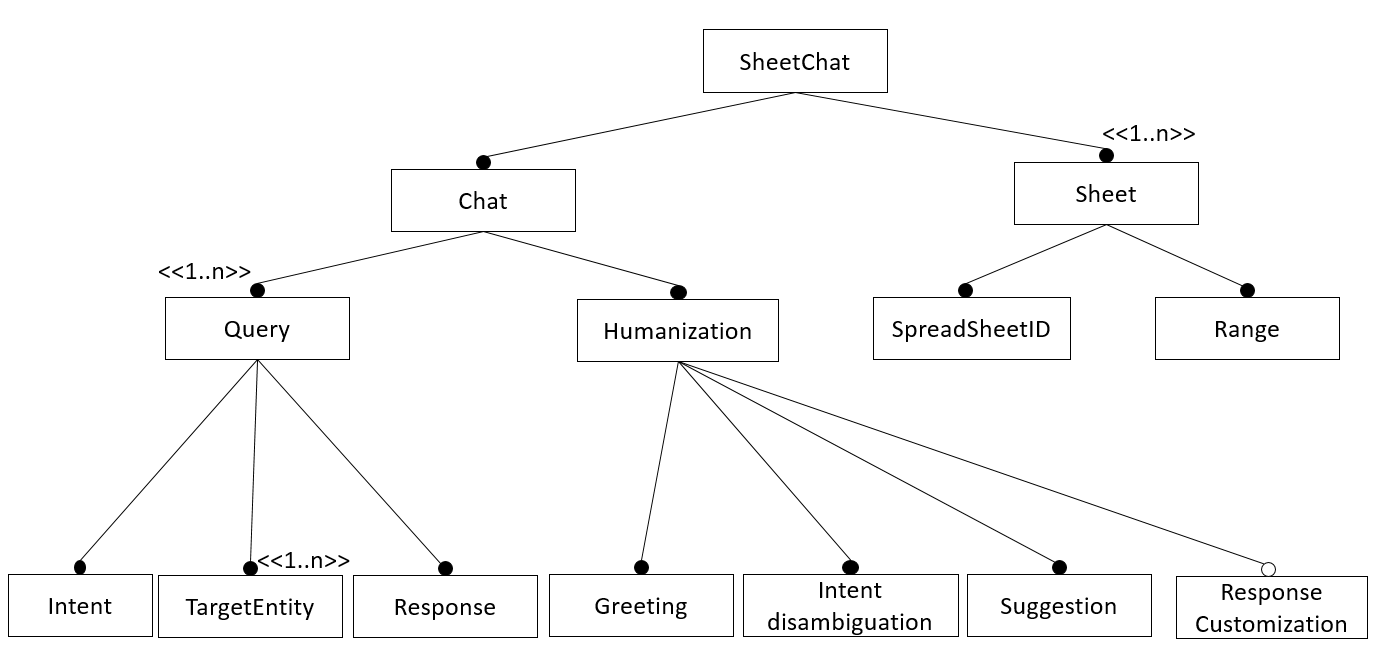
\includegraphics[width=0.8\textwidth]{./figs/FeatureModel.png}
	\caption{Modelo de características de SheetChat.}
	\label{fig:FeatureModel}
\end{figure}

\subsection{Sheet}
\label{sec:Sheet}


\subsection{Chat}
\label{sec:Chat}

\subsubsection{Consultas}
\label{sec:Queries}

\subsubsection{Humanización}
\label{sec:Humanization}


\section{Modelo de datos}
\label{sec:DataModel}

\subsection{Metamodelo}
\label{sec:Metamodel}

\subsection{Sintaxis concreta}
\label{sec:ConcreteSyntax}
